
\renewcommand{\thechapter}{6}
\chapter{EXO-200 Analysis and Results from Denoising}
\label{ch:DenoisingResults}

Data analyzed for the present work extends from \textcolor{red}{DATE to DATE}.  In this chapter, sections~\ref{sec:ResultSimulation}-\ref{sec:ResultFitting} describe the basic elements of the EXO-200 analysis.  Section~\ref{sec:ResultResults} will present the results from this set of data.  In section~\ref{sec:ResultComparison} we compare the results obtained using the denoising scheme of chapter~\ref{ch:DenoisingTheory} to the results which would have been obtained without that algorithm applied, and demonstrate that denoising has contributed to the strength of our physics reach.

\section{Simulation}\label{sec:ResultSimulation}

Here we will describe the simulation of radioactive sources in the EXO-200 detector.  We begin by describing the framework for simulating the deposition of energy from primary decay particles into the liquid xenon and surrounding materials.  From there, we continue to describe the simplified electric field model which permits us to model the drift of ionization towards the anode wires.

\subsection{Simulation of Particles using GEANT}

To simulate the deposition of energy from primary decay particles, version 4.9.3p02 of the GEANT software package is used.~\cite{Agostinelli2003250}\cite{1610988}  This package includes a database containing attenuation properties of many common materials as well as detailed decay modes for most radioactive isotopes.  Angular correlations between gammas are not modeled with this version of the software, but that is expected to be a minor detail and will be corrected by upgrading to a newer version of GEANT in the future.  Forbidden beta decays are generated with an incorrect beta spectrum in the default GEANT software; this is addressed by the EXO collaboration by using our own beta spectra where appropriate.

\begin{figure}
\begin{center}
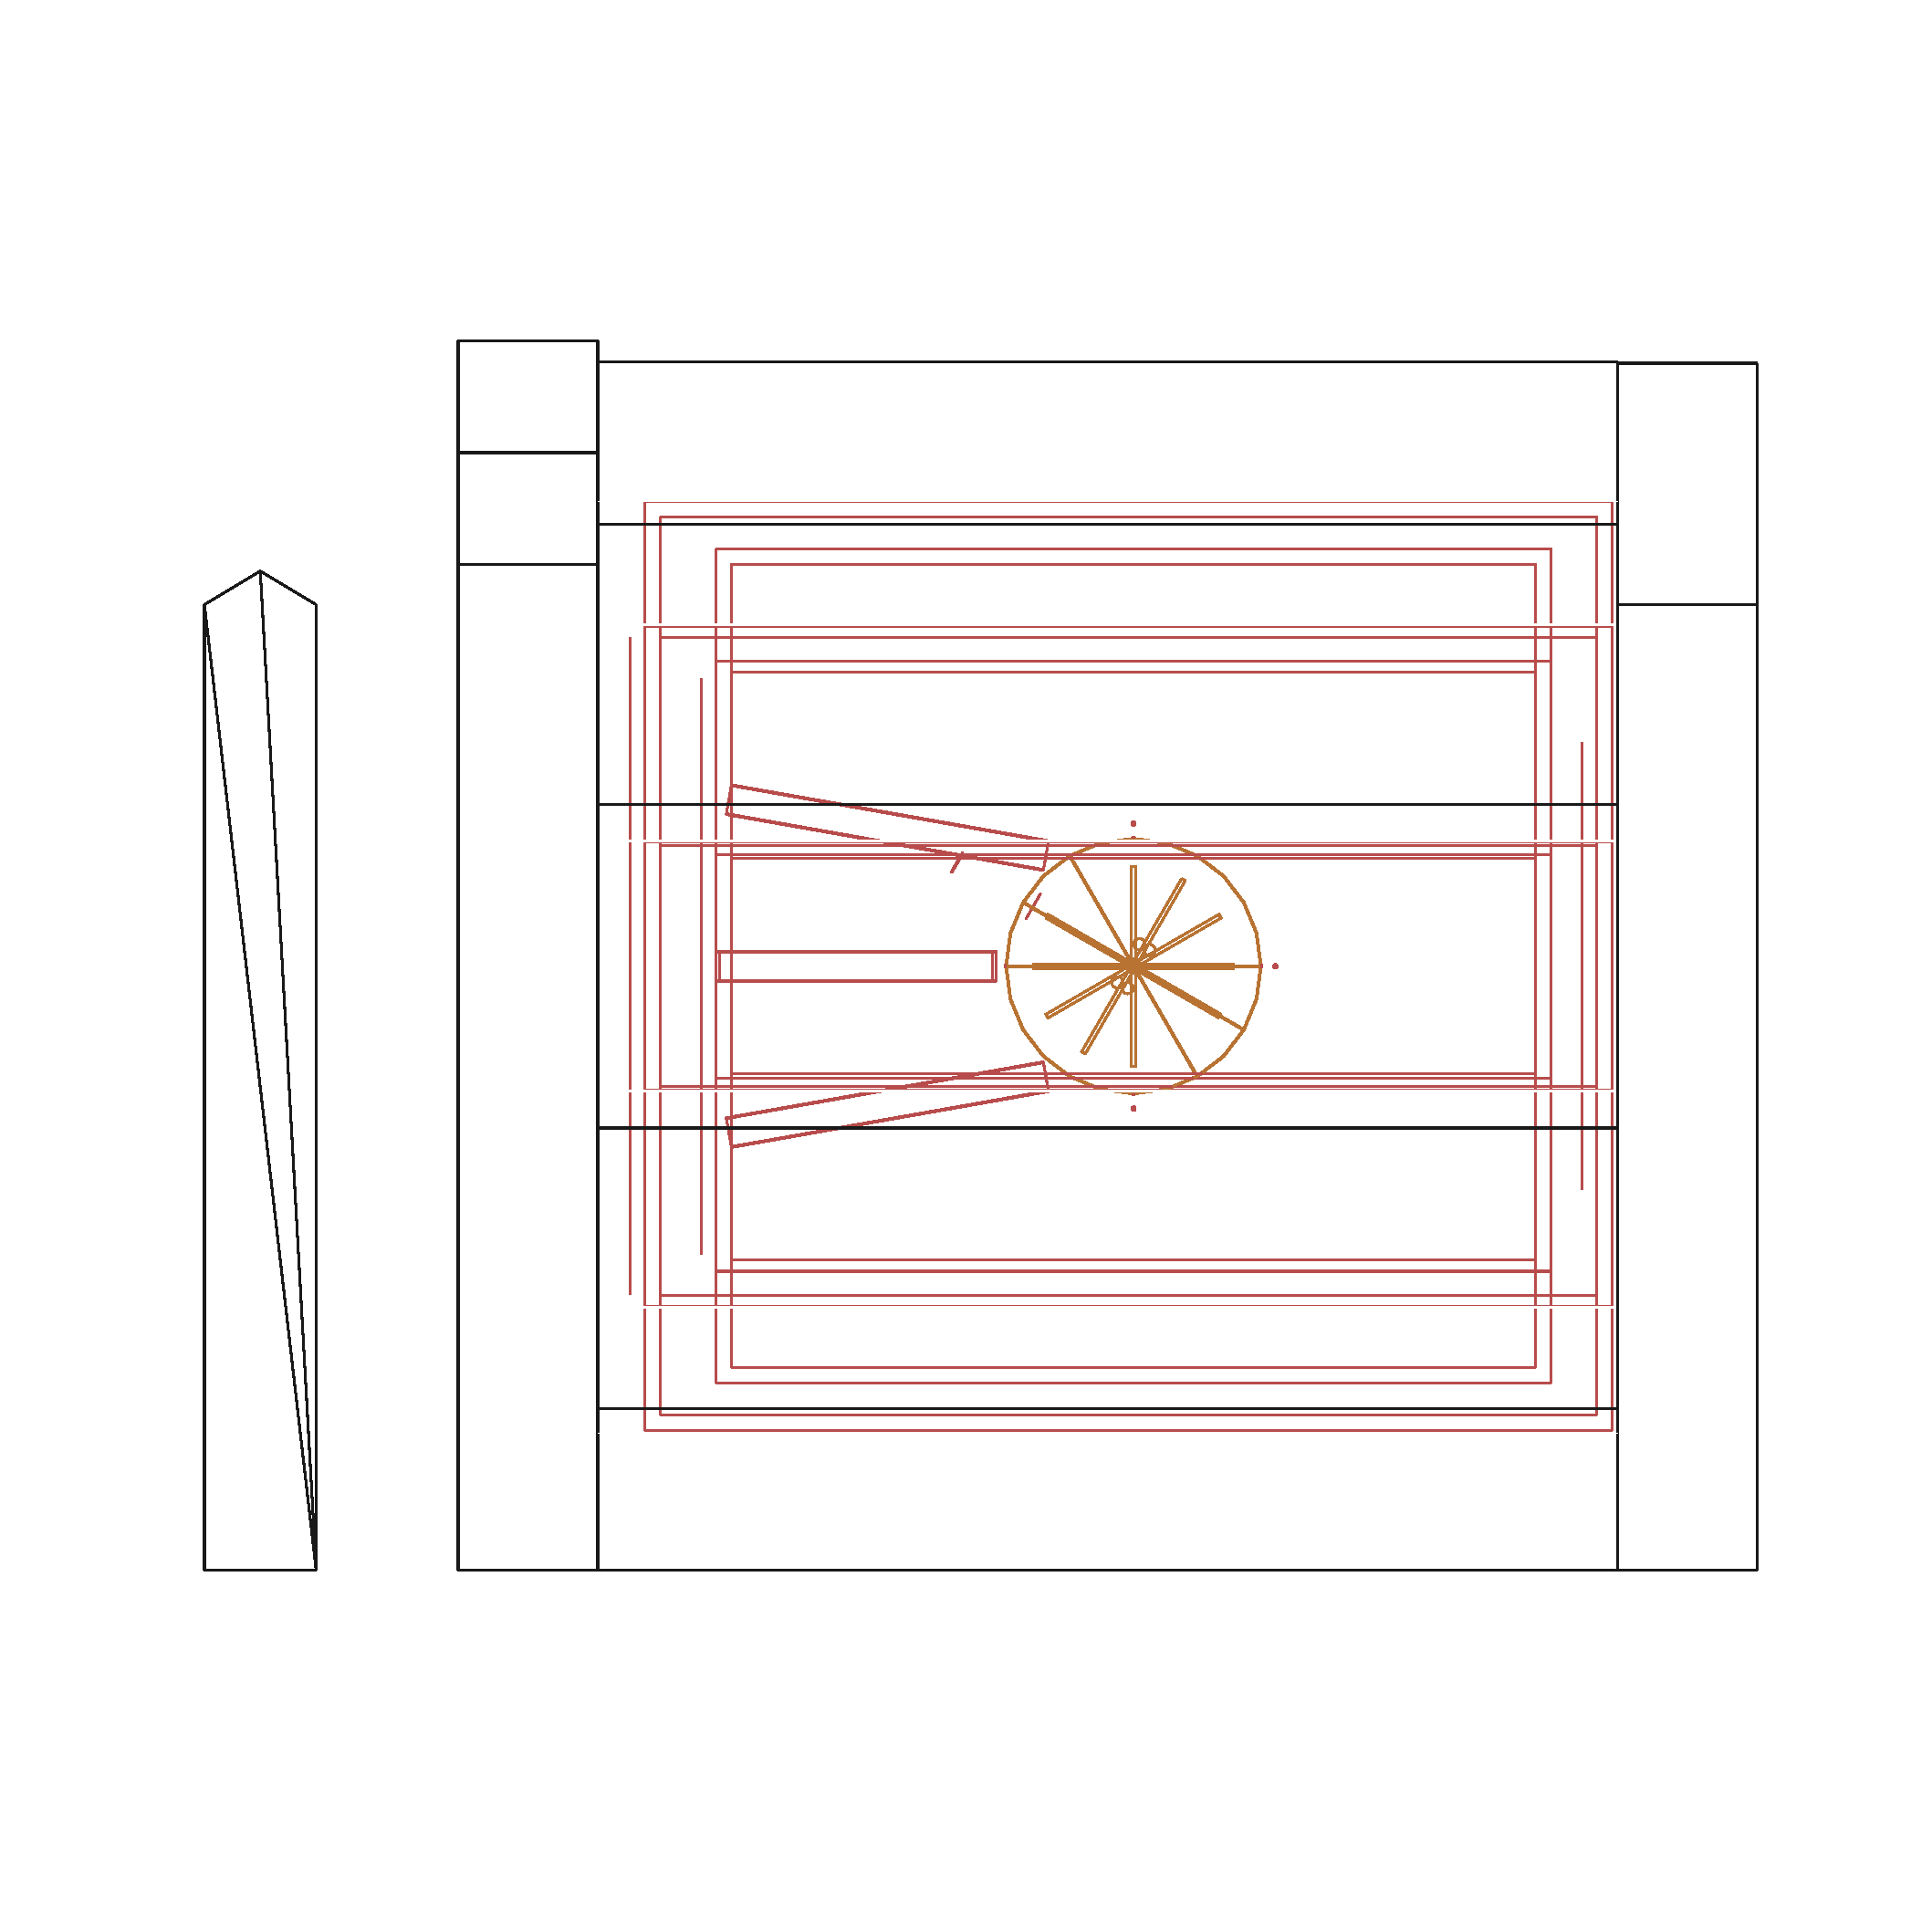
\includegraphics[keepaspectratio=true,width=\textwidth]{OGL_wireframe.eps}
\end{center}
\renewcommand{\baselinestretch}{1}
\small\normalsize
\begin{quote}
\caption{The GEANT simulation includes large-scale features of the EXO-200 detector, including the outer and inner lead wall (black), outer and inner cryostat and TPC legs (red), and the TPC itself (brown).  Components are assembled from simple geometrical shapes, and distant objects are only described coarsely.~\cite{MCDocumentRun2a}}
\label{fig:OGL_wireframevis}
\end{quote}
\end{figure}
\renewcommand{\baselinestretch}{2}
\small\normalsize

\begin{figure}
\begin{center}
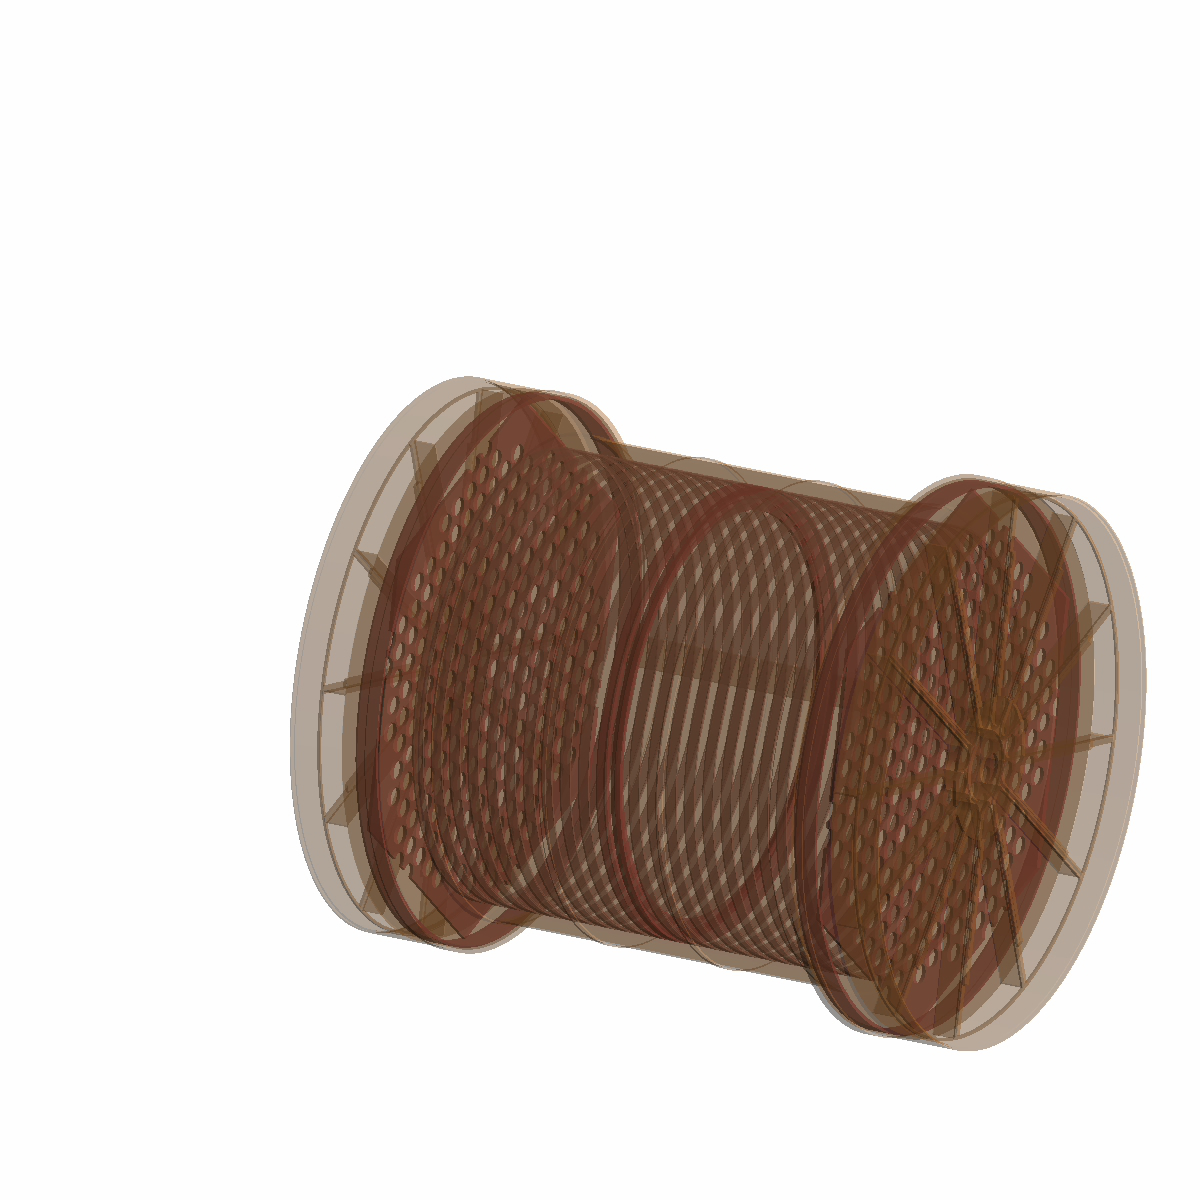
\includegraphics[keepaspectratio=true,width=\textwidth]{TPC_Cu_RayTracer.png}
\end{center}
\renewcommand{\baselinestretch}{1}
\small\normalsize
\begin{quote}
\caption{Detector components which are close to the liquid xenon are simulated in GEANT with far greater accuracy than distant objects, to reduce computational time.~\cite{MCDocumentRun2a}}
\label{fig:RayTracer_TPConly}
\end{quote}
\end{figure}
\renewcommand{\baselinestretch}{2}
\small\normalsize

A model of the EXO-200 detector is simulated in GEANT with a collection of simple geometric volumes, which can be composed to form more complicated structures.  Simulation speed decreases as more volumes are generated, and we expect that it is unimportant to simulate details much smaller than the distance between the detail and the liquid xenon.  We attempt to find a balance between accurate modeling of detailed features and simplification of distant features.  In figure~\ref{fig:OGL_wireframevis} we see the full geometry described in GEANT, where distant objects are constructed from a small number of geometric pieces.  Figure~\ref{fig:RayTracer_TPConly} shows how the TPC is described in GEANT, and we can see the level of detail is much greater.

To simulate particles, GEANT uses a Monte Carlo method.  It models particles as taking a sequence of steps, where each step is randomly generated; the probability distribution of each choice of step is determined by known properties of the particle, the energy of the particle, and the properties of the attenuating material.  The precise set of physical processes which determine the probability distribution is user-selected, and in EXO-200 has been chosen to include all processes which are significant within our energy range of 10 keV to 10 MeV.~\cite{MCDocumentRun2a}

Only energy which deposits in the liquid xenon is observable.  When primary decays are simulated far from the detector, it may be that most of those simulated events deposit no energy in the liquid xenon and are not observable; the simulation must continue running until a sufficient number of simulated events deposit energy in the liquid xenon.  This means that sources which are farther from the liquid xenon require significantly more computational time to accumulate a usable number of statistics.  We find that sources outside of the HFE are subject to $4.5$ attenuation lengths before reaching the liquid xenon, and events reaching the liquid xenon from the inner cryostat can only be simulated at $0.01$ Hz/core by this approach.~\cite{MCDocumentRun2a}

To improve this rate, importance sampling is employed for distant sources.  This approach consists of the following techniques to magnify statistics from a fixed simulation time:
\begin{itemize}
\item Low-energy beta and alpha particles outside of the TPC may be ``killed'', or prematurely eliminated from the simulation based on an expectation that they will not deliver any energy to the liquid xenon.
\item The detector is surrounded by importance sampling ``boundaries'': when a particle passes into a boundary it may be cloned (with a user-selected probability), where the rate of cloning is tracked by a corresponding decrease in particle ``weight.''
\item To avoid biasing the spectrum, it is also necessary to kill particles which pass out of a boundary with the same probability, and increase their weight accordingly.
\end{itemize}
This approach has the effect of using GEANT to simulate the properties of particles reaching the outermost boundary; then draw samples from that distribution and simulate the properties of particles reaching the next boundary; and so forth, amplifying the impact of statistics at each stage.  Further details on this approach can be found in~\cite{Dressel:642987}; it has the effect of increasing simulation speeds from the inner cryostat from $0.01$ Hz/core to a few Hz/core, and makes simulations of backgrounds from outside the lead wall feasible.~\cite{MCDocumentRun2a}

\begin{figure}
\begin{center}
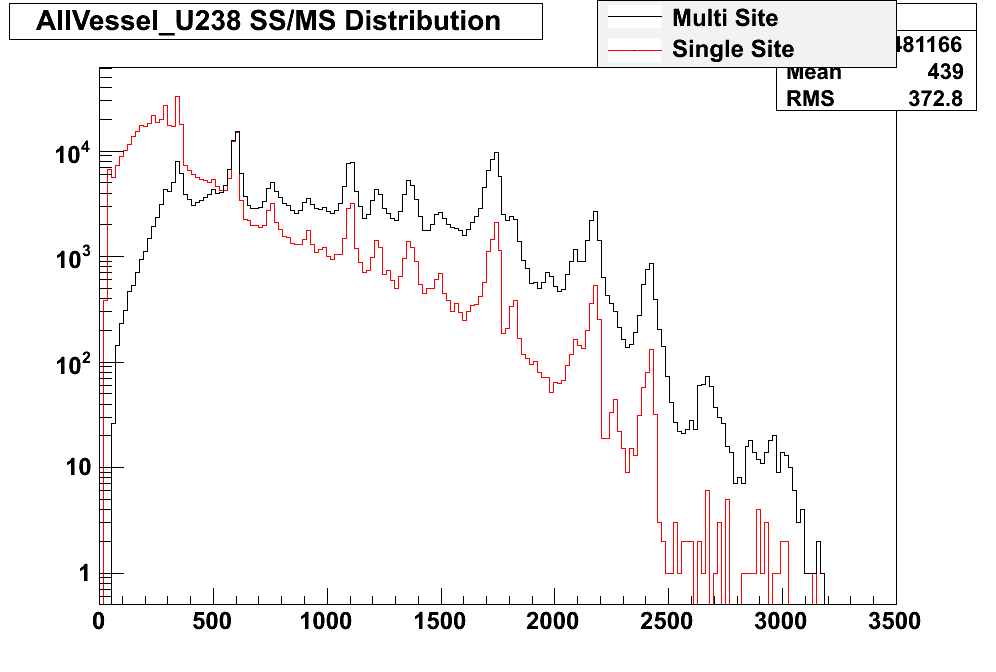
\includegraphics[keepaspectratio=true,width=\textwidth]{AllVessel_U238_single_multi_site_spec.png}
\end{center}
\renewcommand{\baselinestretch}{1}
\small\normalsize
\begin{quote}
\caption{Energy spectra from $^{238}$U in the TPC vessel; single-site and multi-site energy spectra are shown separately.~\cite{MCDocumentRun2a}}
\label{fig:UGeantSpectra}
\end{quote}
\end{figure}
\renewcommand{\baselinestretch}{2}
\small\normalsize

\begin{figure}
\begin{center}
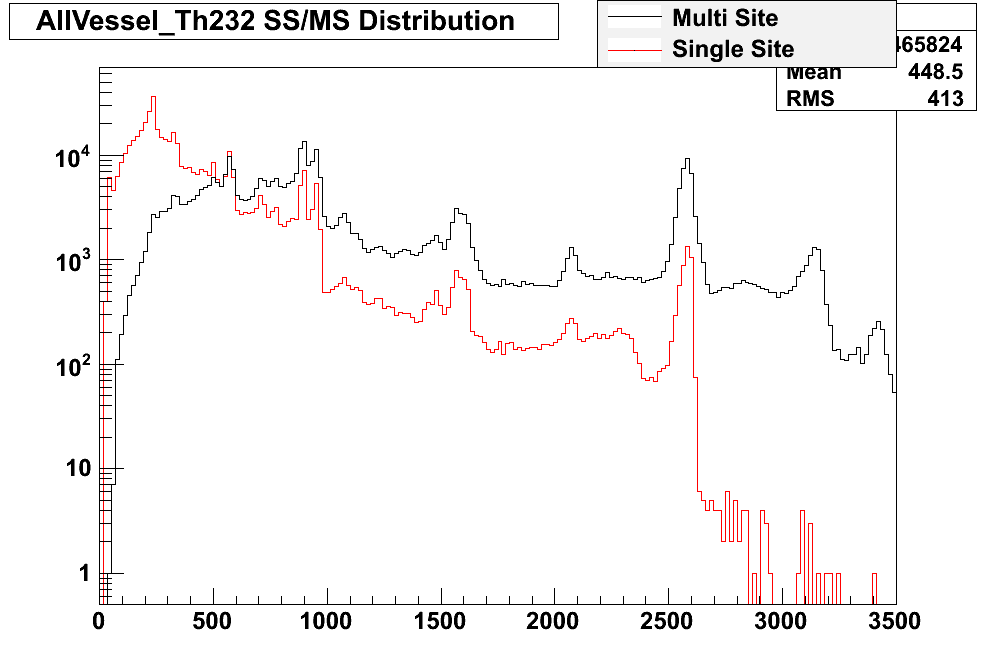
\includegraphics[keepaspectratio=true,width=\textwidth]{AllVessel_Th232_single_multi_site_spec.png}
\end{center}
\renewcommand{\baselinestretch}{1}
\small\normalsize
\begin{quote}
\caption{Energy spectra from $^{232}$Th in the TPC vessel; single-site and multi-site energy spectra are shown separately.~\cite{MCDocumentRun2a}}
\label{fig:ThGeantSpectra}
\end{quote}
\end{figure}
\renewcommand{\baselinestretch}{2}
\small\normalsize

The result of these GEANT simulations is a measurement of the efficiency with which events from various sources reach the liquid xenon, and also an understanding of the energy and position distributions of energy deposits from these sources.  Representative spectra of our primary backgrounds, $^{238}$U and $^{232}$Th, are shown in figures~\ref{fig:UGeantSpectra} and \ref{fig:ThGeantSpectra} respectively.

\subsection{Digitization of Waveforms}

After energy deposits are simulated using GEANT, it is necessary to model the conversion of those energy deposits into collection of scintillation and ionization, and then the generation of digitized waveforms resembling the waveforms which are collected in real data.

To generate a scintillation signal, a purely empirical model is used to estimate the relative signal magnitudes on the north and south APD planes.  This model only takes into account $Z$-dependence of the light collection, and does not incorporate the different light yields expected on each individual APD channel.  This model is therefore rather crude, and can only be used as a rough check on the signal-finding efficiency for scintillation as a function of energy.  Attempts to track optical photons in the TPC have met with only partial success which is insufficient to justify their significant computational cost.  Thus, the EXO simulations are unable to model most aspects of scintillation signals.  Section~\ref{sec:ResultFitting} will describe the methods used to cope with this aspect of simulation.

\begin{figure}
\begin{center}
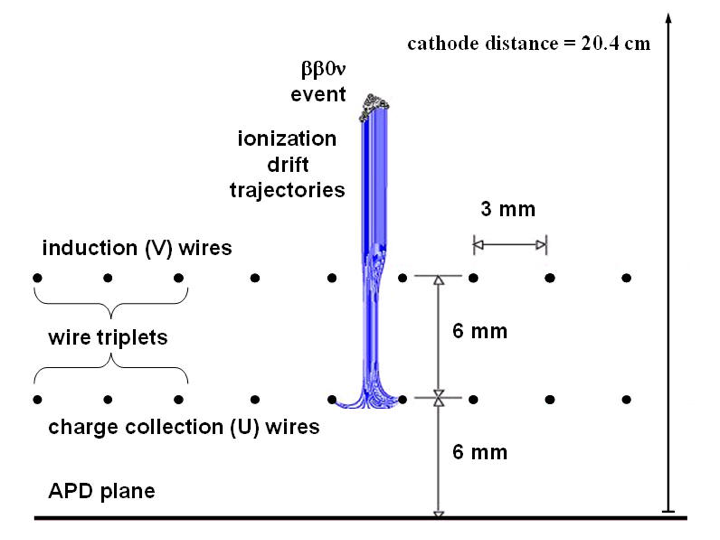
\includegraphics[keepaspectratio=true,width=\textwidth]{ChargeDrift2DModel.png}
\end{center}
\renewcommand{\baselinestretch}{1}
\small\normalsize
\begin{quote}
\caption{The wire planes are modeled in only two dimensions; charge drifts along the field lines, which are arranged to terminate only on the u-wires.~\cite{MCDocumentRun2a}}
\label{fig:TwoDimensionalWireModel}
\end{quote}
\end{figure}
\renewcommand{\baselinestretch}{2}
\small\normalsize

Simulation of charge signals is better-understood.  The detector is modeled by a two-dimensional geometry where, rather than one-dimensional wires arranged in two-dimensional planes, we have wire ``points'' at fixed voltage which are grouped in a one-dimensional pattern.  The v-wires are treated as stacked directly on top of the u-wires; it is impossible to model the true orientation of the v-wires which is rotated relative to the u-wires, but this has generally proven to be a negligible detail for us.  Only one TPC half is modeled because of the approximate mirror symmetry of the detector across the cathode.  Only a few wires are simulated in the second dimension because the electrostatic effect of any one wire will not extend beyond a few wire spacings.  This model is illustrated in figure~\ref{fig:TwoDimensionalWireModel}.~\cite{MCDocumentRun2a}

Electrostatic effects are simulated using the ANSYS Maxwell field simulator.  To simulate the electric fields in the detector, wires are treated as circles with a radius matching the approximate radii of the physical wires, with a constant voltage on their surfaces.  The APD plane and cathode plane are treated as constant-voltage boundaries, and a periodic boundary condition is established on the two remaining boundaries of the model geometry.

These electric fields can be used to trace the paths followed by charge deposits in the detector.  Charge deposits are drifted in small steps based on the direction of the electric field.  The speed of drift is taken from external measurements rather than from the magnitude of the electric field; in most of the bulk of xenon, the electric field and drift velocity are treated as constant, but near the u-wire plane the drift velocity is increased slightly to account for higher electric fields experienced in that region of the detector.  Charge attenuation due to finite purity can be modeled at this step, but generally is treated as infinite here; charge diffusion effects are ignored.

\begin{figure}
\begin{center}
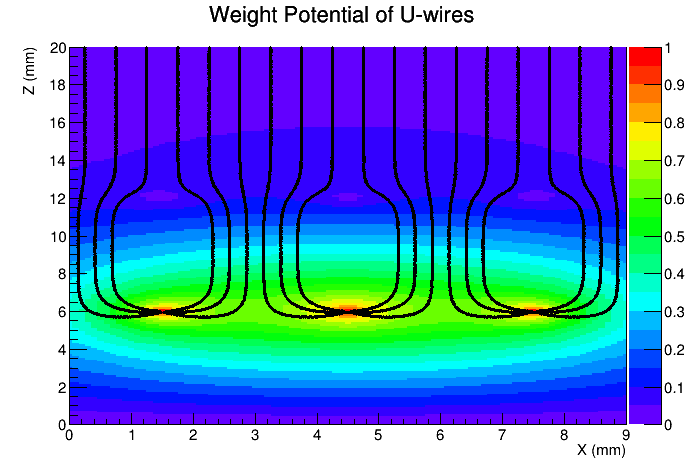
\includegraphics[keepaspectratio=true,width=\textwidth]{WeightPotContoursU_WithE.png}
\end{center}
\renewcommand{\baselinestretch}{1}
\small\normalsize
\begin{quote}
\caption{Weight potential of a u-wire channel consisting of three ganged wires.  Electric field lines are superimposed.~\cite{MCDocumentRun2a}}
\label{fig:UWireWeightPotential}
\end{quote}
\end{figure}
\renewcommand{\baselinestretch}{2}
\small\normalsize

\begin{figure}
\begin{center}
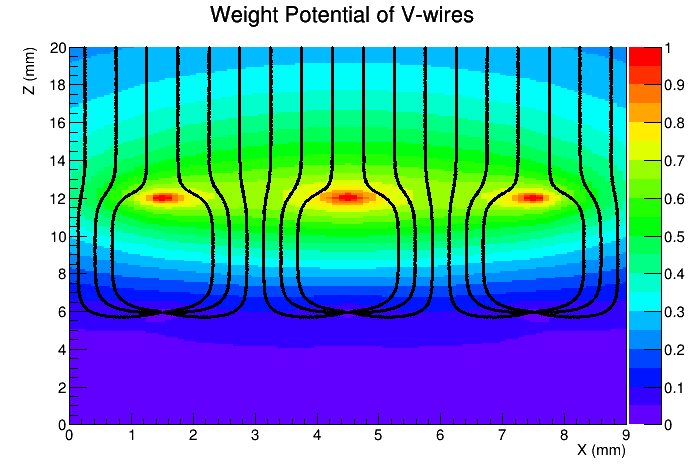
\includegraphics[keepaspectratio=true,width=\textwidth]{WeightPotContoursV_WithE.png}
\end{center}
\renewcommand{\baselinestretch}{1}
\small\normalsize
\begin{quote}
\caption{Weight potential of a v-wire channel consisting of three ganged wires.  Electric field lines are superimposed.~\cite{MCDocumentRun2a}}
\label{fig:VWireWeightPotential}
\end{quote}
\end{figure}
\renewcommand{\baselinestretch}{2}
\small\normalsize

We have discussed in section~\ref{sec:DetectorReadout} that charge is induced on the u-wires and v-wires; this means that we must record the amount of charge induced at each step along the drift path of the charge deposit.  This is done based on the Shockley-Ramo Theorem, which states that the change in induced charge $\delta q_i$ on an electrode $i$ is equal to:
\begin{equation}
\delta q_i = Q \delta W_i,
\end{equation}
where $Q$ is the total drifting charge and $W_i$ is the weighting potential of electrode $i$, defined as the potential which would be induced in our geometry if the potential on electrode $i$ were set to $1$ and the potential on all other boundaries were set to $0$.~\cite{ShockleyPaper}\cite{1686997}  Figures~\ref{fig:UWireWeightPotential} and~\ref{fig:VWireWeightPotential} illustrate the weighting potentials of a u-wire and v-wire channel, respectively.

Finally, the functions of integrated charge versus time must be converted to shaped digitized waveforms, and noise must be added.  The shaping and gain amplification is performed to match the electronics described in section~\ref{sec:DetectorReadout}.  To ensure accurate time shaping, the functions are all sampled at a bandwidth of $10$ MHz, and then downsampled after shaping to the nominal $1$ MHz.  Digitization is performed by converting voltages into units of ADC counts, then truncating to an integer value.  To model saturation effects, this number is pulled into the integer range $[0, 4096)$.

\begin{figure}
\begin{center}
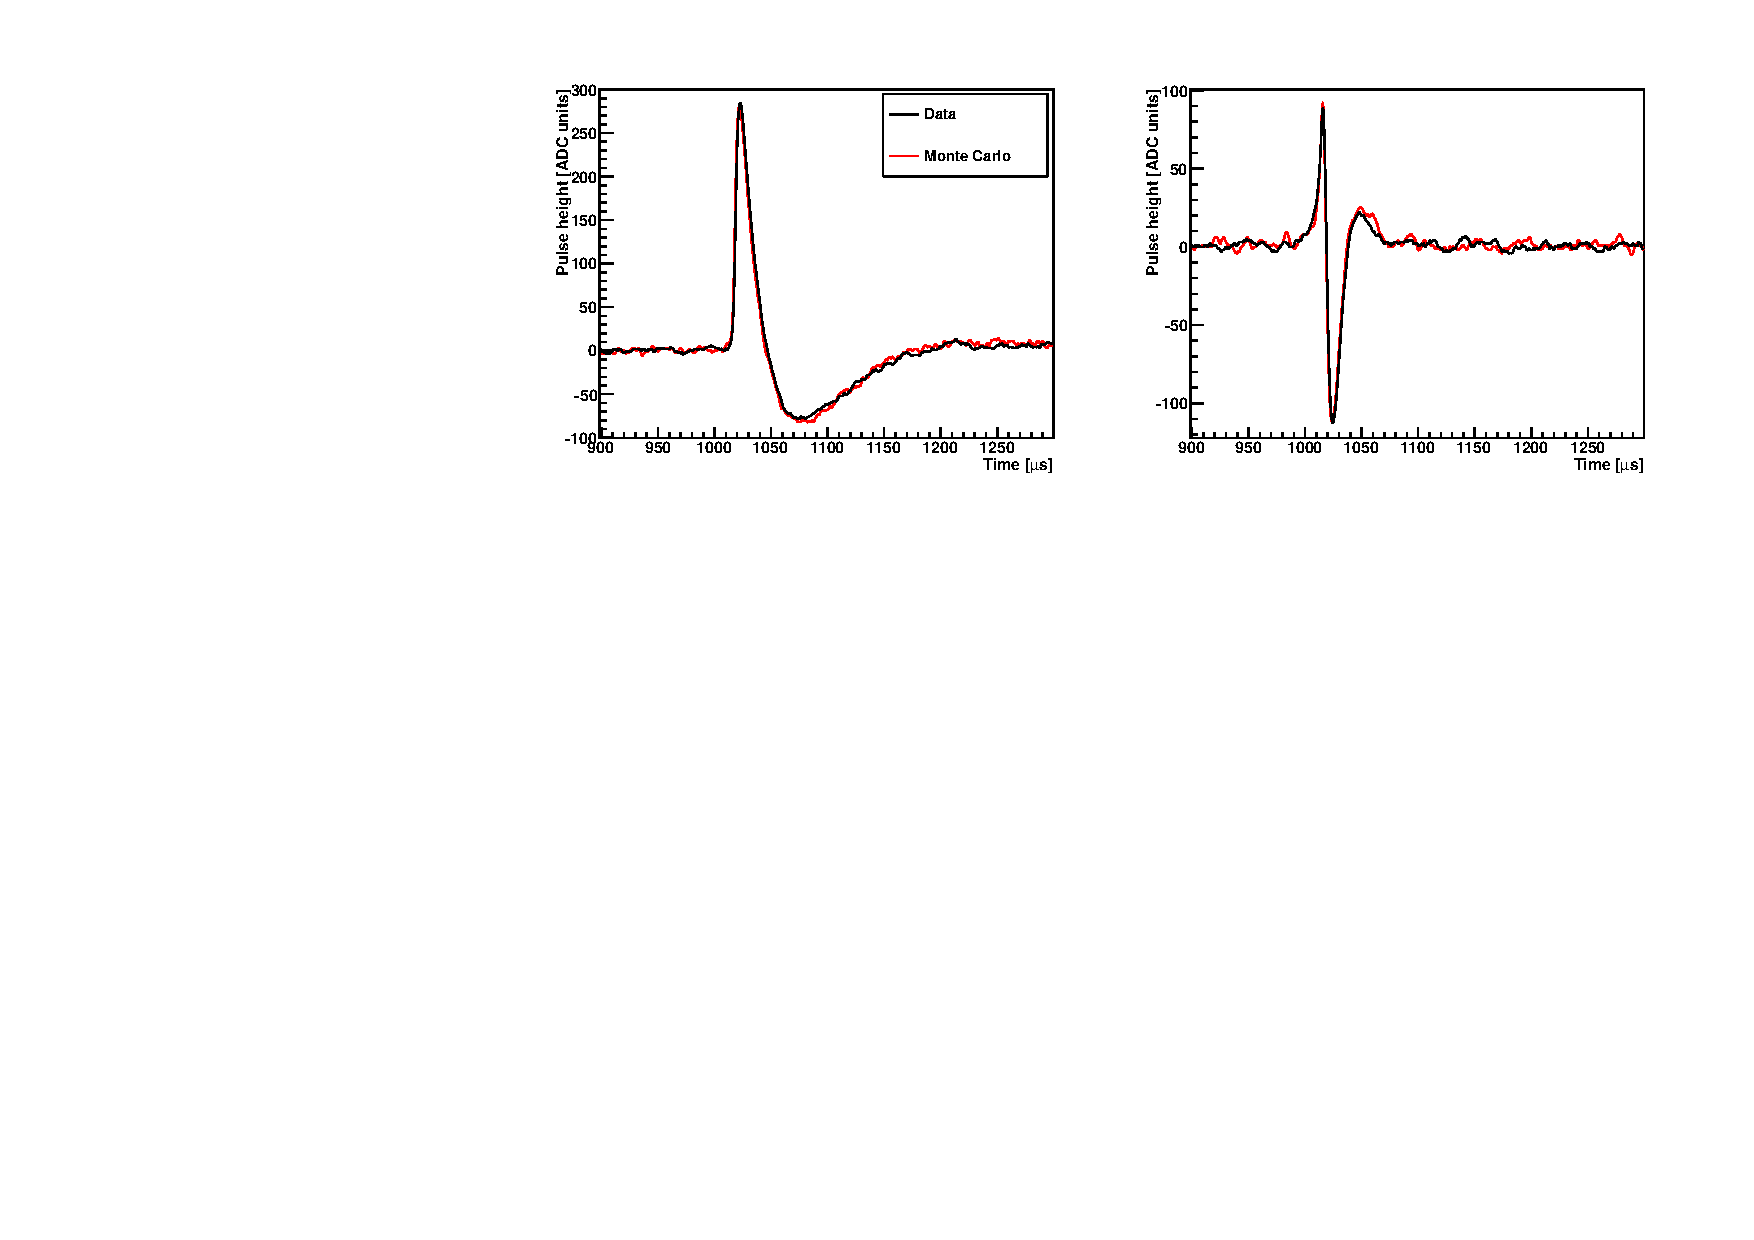
\includegraphics[keepaspectratio=true,width=\textwidth]{pulse_comp.pdf}
\end{center}
\renewcommand{\baselinestretch}{1}
\small\normalsize
\begin{quote}
\caption{Comparison between simulated and observed waveforms on a u-wire (left) and v-wire (right) from $^{228}$Th sources.  The events are chosen to have similar energies so that the magnitudes match.~\cite{MCDocumentRun2a}}
\label{fig:MCPulseComparison}
\end{quote}
\end{figure}
\renewcommand{\baselinestretch}{2}
\small\normalsize

Finally, we have found that the most effective way to add electronic noise to the signals is by extracting a set of representative noise waveforms from real data.  These are taken from a large number of solicited triggers which have been checked for the absence of a coincident event.  To increase the number of noise signals available, the noise waveforms sampled from the detector are spliced together, and simulated events may draw their noise from any subrange of the spliced-together noise waveform.  This method has been found to agree better with data than noise simulations using a random-number generator.  Figure~\ref{fig:MCPulseComparison} compares waveforms observed from a sample event in data and simulation.~\cite{MCDocumentRun2a}

\begin{figure}
\begin{center}
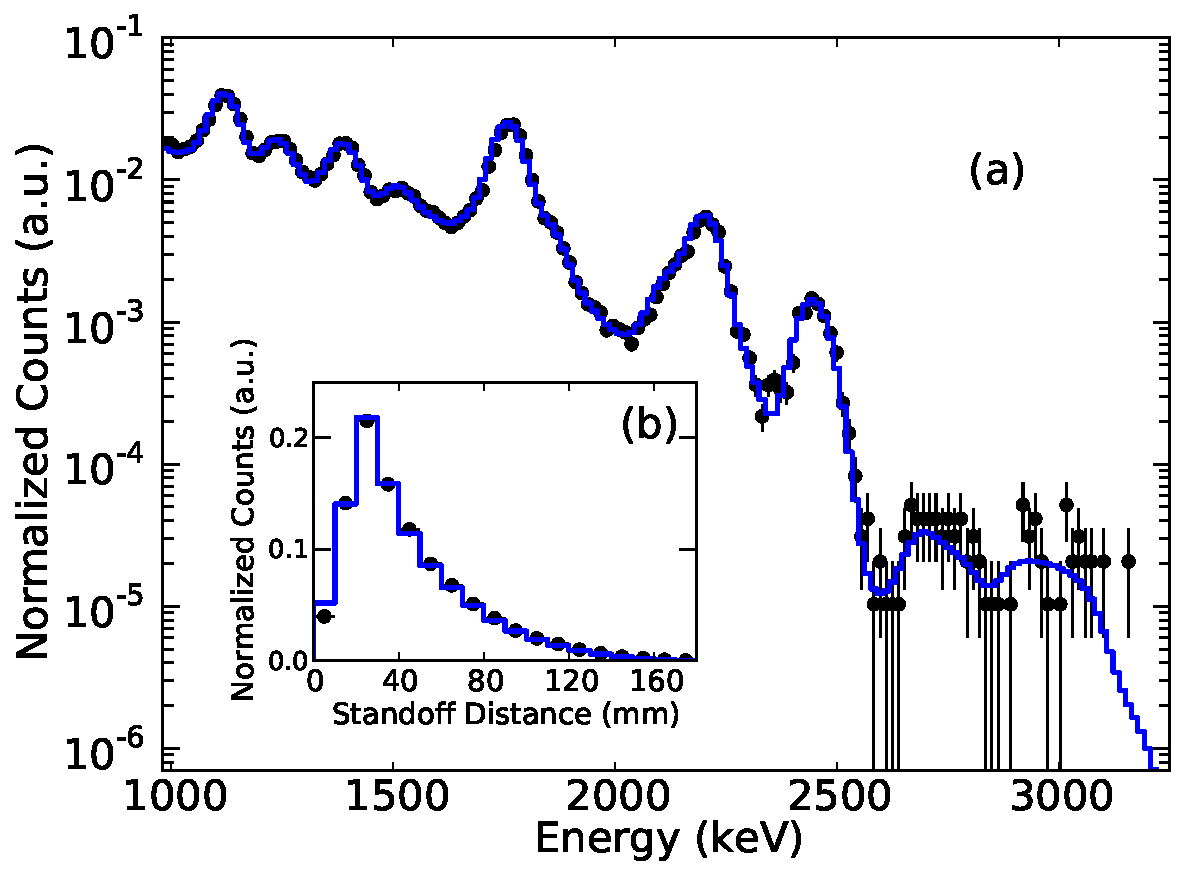
\includegraphics[keepaspectratio=true,width=\textwidth]{SS_Ra226_Campaign7.pdf}
\end{center}
\renewcommand{\baselinestretch}{1}
\small\normalsize
\begin{quote}
\caption{Comparison between simulated and observed energy spectra (a) and standoff distance (b) in single-site $^{226}$Ra events from a source located at position S5.~\cite{NewEXObb0nPaper_2014}}
\label{fig:RaSourceMCComparison}
\end{quote}
\end{figure}
\renewcommand{\baselinestretch}{2}
\small\normalsize

In this way, we are able to generate simulated data which in most respects resembles real data collected from the detector.  The EXO-200 simulation has shown remarkable agreement with the detector in the properties of energy and cluster location, as illustrated in figure~\ref{fig:RaSourceMCComparison}.  A significant effort has been made to achieve excellent agreement between simulation and data, and the result is that we can claim a strong understanding of the behavior of the EXO-200 detector.

\section{Reconstruction}\label{sec:ResultReconstruction}


\section{Energy Corrections}\label{sec:ResultEnergy}

\subsection{Charge Corrections}\label{sec:ResultEnergyCharge}

\subsection{Light Corrections}\label{sec:ResultEnergyLight}

\section{Fitting}\label{sec:ResultFitting}

\section{Results and Physics Reach}\label{sec:ResultResults}

\section{Comparison to Results without Denoising}\label{sec:ResultComparison}

\section{Summary}\label{sec:ResultSummary}
